\icode[magenta]{N20-MD-CA-L4-261111-001}
\nceeID[20]{2020全国\Rmnum{2}}{25}
如图，一竖直圆管质量为\(M\)，下端距水平地面的高度为\(H\)，顶端塞有一质量为\(m\)的小球。圆管由静止自由下落，与地面发生多次弹性碰撞，且每次碰撞时间均极短；在运动过程中，管始终保持竖直。已知\(M = 4m\)，球和管之间的滑动摩擦力大小为\(4mg\)， \(g\)为重力加速度的大小，不计空气阻力。
\begin{enumerate}
	\item 求管第一次与地面碰撞后的瞬间，管和球各自的加速度大小；
	\item 管第一次落地弹起后，在上升过程中球没有从管中滑出，求管上升的最大高度；
	\item 管第二次落地弹起的上升过程中，球仍没有从管中滑出，求圆管长度应满足的条件。
\end{enumerate}

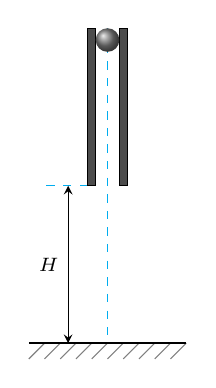
\begin{tikzpicture}[>=stealth,font=\scriptsize]
	\draw[dashed,cyan] (0,4)--(0,0) (-.25,2)--(-.8,2);
	\draw[fill=gray!60!black] (-.15,2) rectangle(-.25,4) (.15,2) rectangle(.25,4);
	\shade[ball color=gray] (0,3.85) circle(.15);
	\draw[<->,thin] (-.5,0)--node[left]{\(H\)}(-.5,2);
	\foreach \x in {-1,-.8,...,.8}
		\draw[gray] (\x,-.2)--++(.2,.2);
	\draw[thick] (-1,0)--(1,0);
\end{tikzpicture}
\begin{answer}
	（1）\(a_1 = 2g\)、\(a_2 = 3g\)（2）\(\frac{13}{25}H\)（3）\(L \geq \frac{152}{125}H\)
	
	提示：与地面接触之前管和球相对静止

	\begin{tikzpicture}[>=stealth,font=\scriptsize]
		\draw[->,blue] (-.5,0)--(3.5,0)node[below]{\(t\)};
		\node at(0,0)[below left]{\(O\)};
		\draw[->,blue] (0,-2.5)--(0,2.5)node[right]{\(v\)};
		\draw[magenta] (0,2)node[left,blue]{\(v_1\)}--(1.6,.4);
		\draw[brown] (0,-2)node[left,blue]{\(- v_1\)}--(1.6,.4);
		\draw[dashed,cyan] (0,.4)node[left,blue]{\(\frac{1}{5}v_1\)}--(1.6,.4)--(1.6,0)node[below,blue]{\(\frac{2v_1}{5g}\)};
		\draw[teal] (1.6,.4)--(2.4,0)node[below,blue]{\(\frac{3v_1}{5g}\)};
		\node at(1.5,-2.5){第一次落地弹起};
	\end{tikzpicture}
	\begin{tikzpicture}[>=stealth,font=\scriptsize]
		\draw[->,blue] (-.5,0)--(3.5,0)node[below]{\(t\)};
		\node at(0,0)[below left]{\(O\)};
		\draw[->,blue] (0,-2.5)--(0,2.5)node[right]{\(v\)};
		\draw[magenta] (0,1.5)node[left,blue]{\(v_2\)}--(1.2,.3);
		\draw[brown] (0,-2)node[left,blue]{\(- v_2\)}--(1.2,.3);
		\draw[dashed,cyan] (0,.3)node[left,blue]{\(\frac{1}{5}v_2\)}--(1.2,.3)--(1.2,0)node[below,blue]{\(\frac{2v_2}{5g}\)};
		\draw[teal] (1.2,.3)--(1.6,0)node[below right,blue]{\(\frac{3v_2}{5g}\)};
		\node at(1.5,-2.5){第二次落地弹起};
	\end{tikzpicture}
\end{answer}